% Options for packages loaded elsewhere
\PassOptionsToPackage{unicode}{hyperref}
\PassOptionsToPackage{hyphens}{url}
\PassOptionsToPackage{dvipsnames,svgnames*,x11names*}{xcolor}

%%%%%%%%%%%%%%%%%%%%%%%%%%%%%%%%%%%%%%%%%%%%%%%%%%%%%%%%%%%%%%%%%%%%%%%%%%%%%%%%% 
\documentclass[
  10pt,
  french,
  a4paper,
  DIV=18]{scrartcl}

\usepackage{fontawesome} %! Icones (à charger en premier sinon ca plante)

%%%%%%%%%%%%%%%%%%%%%%%%%%%%%%%%%%%%%%%%%%%%%%%%%%%%%%%%%%%%%%%%%%%%%%%%%%%%%%%%%
%% Réglages Beamer

%%%%%%%%%%%%%%%%%%%%%%%%%%%%%%%%%%%%%%%%%%%%%%%%%%%%%%%%%%%%%%%%%%%%%%%%%%%%%%%%%
% Fontes
\usepackage{fontspec} % Polices texte (latin modern par défaut)
\defaultfontfeatures{Scale=MatchLowercase}
\defaultfontfeatures[\rmfamily]{Ligatures=TeX,Scale=1}
  \setmonofont[Scale = MatchLowercase]{DejaVu Sans Mono}

\usepackage{amsmath}		% Commandes essentielles
\usepackage{amssymb}		% Principaux symboles
\usepackage{unicode-math} % Polices maths (charger les paquets maths avant!)
  \setmathfont[]{latinmodern-math.otf}

%%%%%%%%%%%%%%%%%%%%%%%%%%%%%%%%%%%%%%%%%%%%%%%%%%%%%%%%%%%%%%%%%%%%%%%%%%%%%%%%%
% Thèmes Beamer

%%%%%%%%%%%%%%%%%%%%%%%%%%%%%%%%%%%%%%%%%%%%%%%%%%%%%%%%%%%%%%%%%%%%%%%%%%%%%%%%%
% use microtype if available
\IfFileExists{microtype.sty}{
  \usepackage[]{microtype}
  \UseMicrotypeSet[protrusion]{basicmath} % disable protrusion for tt fonts
}{}

%%%%%%%%%%%%%%%%%%%%%%%%%%%%%%%%%%%%%%%%%%%%%%%%%%%%%%%%%%%%%%%%%%%%%%%%%%%%%%%%%
% Couleurs
\usepackage{xcolor}
\definecolor{green}{rgb}{0, 0.6, 0} % le vert de base est trop brillant!

%%%%%%%%%%%%%%%%%%%%%%%%%%%%%%%%%%%%%%%%%%%%%%%%%%%%%%%%%%%%%%%%%%%%%%%%%%%%%%%%%
% Liens et métadonnées PDF
\IfFileExists{url.sty}{\usepackage{url}}{} % add URL line breaks if available
\IfFileExists{bookmark.sty}{\usepackage{bookmark}}{\usepackage{hyperref}}
\hypersetup{
  pdftitle={MPSI 1 - DS9 - Thermodynamique},
  colorlinks=true,
  linkcolor=Blue,
  filecolor=Blue,
  citecolor=Blue,
  urlcolor=Blue,
}

%%%%%%%%%%%%%%%%%%%%%%%%%%%%%%%%%%%%%%%%%%%%%%%%%%%%%%%%%%%%%%%%%%%%%%%%%%%%%%%%%
% Marges avec packages geometry

%%%%%%%%%%%%%%%%%%%%%%%%%%%%%%%%%%%%%%%%%%%%%%%%%%%%%%%%%%%%%%%%%%%%%%%%%%%%%%%%%
% Coloration syntaxique



%%%%%%%%%%%%%%%%%%%%%%%%%%%%%%%%%%%%%%%%%%%%%%%%%%%%%%%%%%%%%%%%%%%%%%%%%%%%%%%%%
% Tableaux
\usepackage{array,tabularx,longtable,booktabs}
\usepackage{colortbl} % colorier les cellules d'un tableau
% Correct order of tables after \paragraph or \subparagraph
\usepackage{etoolbox}
\makeatletter
\patchcmd\longtable{\par}{\if@noskipsec\mbox{}\fi\par}{}{}
\makeatother
% Allow footnotes in longtable head/foot
\IfFileExists{footnotehyper.sty}{\usepackage{footnotehyper}}{\usepackage{footnote}}
\makesavenoteenv{longtable}

%%%%%%%%%%%%%%%%%%%%%%%%%%%%%%%%%%%%%%%%%%%%%%%%%%%%%%%%%%%%%%%%%%%%%%%%%%%%%%%%%
% Réglages généraux
\usepackage{multicol} % Plusieurs colonnes
\usepackage[breakable]{tcolorbox} % Encadrements

\usepackage{cancel} % permet de barrer des termes dans des expressions mathématiques (simplifications)

\usepackage{graphicx}
\usepackage[labelfont={bf,sf},textfont=sf]{caption} % personnalisation des légendes des figures
\usepackage{float}
\makeatletter
\def\maxwidth{\ifdim\Gin@nat@width>\linewidth\linewidth\else\Gin@nat@width\fi}
\def\maxheight{\ifdim\Gin@nat@height>\textheight\textheight\else\Gin@nat@height\fi}
\makeatother
% Scale images if necessary, so that they will not overflow the page
% margins by default, and it is still possible to overwrite the defaults
% using explicit options in \includegraphics[width, height, ...]{}
\setkeys{Gin}{width=\maxwidth,height=\maxheight,keepaspectratio}
% Set default figure placement to H 
\makeatletter
\def\fps@figure{H}
\makeatother


% Texte barré

% prevent overfull lines
\setlength{\emergencystretch}{3em} 

% listes serrées 
\providecommand{\tightlist}{%
  \setlength{\itemsep}{0pt}\setlength{\parskip}{0pt}}

% numérotation des sections
\setcounter{secnumdepth}{3}

%%%%%%%%%%%%%%%%%%%%%%%%%%%%%%%%%%%%%%%%%%%%%%%%%%%%%%%%%%%%%%%%%%%%%%%%%%%%%%%%%
% Langues
\usepackage[shorthands=off,main=french]{babel}
  \frenchsetup{StandardLists=true} % pas de listes à la française


%%%%%%%%%%%%%%%%%%%%%%%%%%%%%%%%%%%%%%%%%%%%%%%%%%%%%%%%%%%%%%%%%%%%%%%%%%%%%%%%%
%% Schémas et graphiques
\usepackage{tikz}            % dessins avec pdfTeX ou luaTeX
\usetikzlibrary{shapes}      % formes géométriques supplémentaires
\usetikzlibrary{angles}      % marquages angles
\usetikzlibrary{quotes}      % nom des angles
\usetikzlibrary{arrows.meta} % flèches variées
\usetikzlibrary{decorations} % décorations de lignes (ondulée, enlacée, ...)
\usetikzlibrary{decorations.fractals}
\usetikzlibrary{calc}		 % Calcul de positions relatives
\usetikzlibrary{mindmap}	 % Cartes mentales

\tikzset{math3d/.style={x= {(-0.353cm,-0.353cm)}, z={(0cm,1cm)},y={(1cm,0cm)}}} % perspective 3D avec z vers le haut
\tikzset{>=latex} % flèches par défaut
\usepackage{pgfplots}        % Tracé de graphes de données expérimentales
\pgfplotsset{compat=default}
\usepackage{keystroke} % Symboles touches clavier français

%%%%%%%%%%%%%%%%%%%%%%%%%%%%%%%%%%%%%%%%%%%%%%%%%%%%%%%%%%%%%%%%%%%%%%%%%%%%%%%%%%%
%% Packages pour la physique-chimie
\usepackage{siunitx}            % unités SI
\sisetup{locale=FR}             % typographie française
\sisetup{inter-unit-product =.} % point entre les unités
\usepackage[european resistor, europeancurrents, straightvoltages]{circuitikz} % dessin de circuits électriques avec conventions européennes sauf pour inductance
\tikzset{mesure/.style={draw,thick,circle,fill=white,minimum size =0.75cm,inner sep=0pt}} % style tikz pour dessiner sur un noeud un cercle de voltmètre ou d'ampèremètre avec la commande node[mesure].
\usepackage{chemfig}           % représentations molécules
\usepackage[version=4]{mhchem} % formules et équations chimiques

%%%%%%%%%%%%%%%%%%%%%%%%%%%%%%%%%%%%%%%%%%%%%%%%%%%%%%%%%%%%%%%%%%%%%%%%%%%%%%%%%%%
% Algorithmes en pseudo-code
\usepackage[french,onelanguage,tworuled]{algorithm2e}
\SetEndCharOfAlgoLine{} % pas de ; à la fin d'une instruction
\let\oldReturn\Return % stocke la définition de la commande \Return dans \oldReturn
\let\Return\undefined % efface la définition de la commande \Return (conflit avec keystroke)
\SetKwComment{cp}{\# }{} % commentaires débutant par # (style python) avec la commande \cp
\newcommand\mycommentfont[1]{\sffamily\textcolor{gray}{#1}} % style des commentaires
\SetCommentSty{mycommentfont}
\newcommand\myKwfont[1]{\bfseries\textcolor{blue}{#1}} % style des mots clefs
\SetKwSty{myKwfont}
\newcommand\myArgfont[1]{\itshape\textcolor{green}{#1}} % style des arguments
\SetArgSty{myArgfont}

%%%%%%%%%%%%%%%%%%%%%%%%%%%%%%%%%%%%%%%%%%%%%%%%%%%%%%%%%%%%%%%%%%%%%%%%%%%%%%%%%
% Commandes perso

% dérivation
\renewcommand{\d}{\mathrm{d}} % d droit en mode math
\newcommand{\derive}[2]{\dfrac{\mathrm{d}#1}{\mathrm{d}#2}}
\newcommand{\derivesec}[2]{\dfrac{\mathrm{d}^2#1}{\mathrm{d}#2^2}}
\newcommand{\deriven}[3]{\dfrac{\mathrm{d}^{#3}#1}{\mathrm{d}#2^{#3}}}
\newcommand{\derivep}[2]{\dfrac{\partial#1}{\partial#2}}


% opérateurs vectoriels
\newcommand{\Grad}{\vec{\mathrm{grad}}} % gradient
\newcommand{\Rot}{\vec{\mathrm{rot}}} % rotationnel
\newcommand{\Div}{\mathrm{div}} % divergence (\div déja défini)

% informatique
\newcommand{\variable}[2]{
\begin{tabular}{|c|c|}
\hline
\cellcolor{gray}\texttt{#1} & \texttt{#2} \\
\hline
\end{tabular}
}

% Icônes FontAwesome
\newcommand{\attention}{\faicon{exclamation-triangle}\:} 
\newcommand{\parcoeur}{\faicon{heart}} 

% Blocs tcolorbox

\newtcolorbox{myblock}[2]{
  title=#1,  
  halign=#2,
  colback=blue!10!white,
  colframe=blue!75!black,
  fonttitle=\sffamily\bfseries,
  }
\newtcolorbox{myalertblock}[2]{
  title=#1,  
  halign=#2,
  colback=red!10!white,
  colframe=red!75!black,
  fonttitle=\sffamily\bfseries,
  }

\newtcolorbox{myexampleblock}[2]{
  title=#1,
  halign=#2,
  colback=green!10!white,
  colframe=green!75!black,
  fonttitle=\sffamily\bfseries,
  }

%%%%%%%%%%%%%%%%%%%%%%%%%%%%%%%%%%%%%%%%%%%%%%%%%%%%%%%%%%%%%%%%%%%%%%%%%%%%%%%%%
%% Page de titre
\title{MPSI 1 - DS9 - Thermodynamique}

\usepackage{etoolbox}
\makeatletter
\providecommand{\subtitle}[1]{% add subtitle to \maketitle
  \apptocmd{\@title}{\par {\large #1 \par}}{}{}
}
\makeatother
\subtitle{Durée 3h / Calculettes autorisées}


\date{2023-2024}



%%%%%%%%%%%%%%%%%%%%%%%%%%%%%%%%%%%%%%%%%%%%%%%%%%%%%%%%%%%%%%%%%%%%%%%%%%%%%%%%%
%% En-tête et pied de page

\usepackage{scrlayer-scrpage} % Titre courant et pied de page perso (compatible KOMA-script)
\pagestyle{scrheadings}
\ihead{Devoirs Surveillés} 
\ohead{MPSI 1 - DS9 - Thermodynamique}
\ifoot{Physique-Chimie MPSI}
\cfoot{\pagemark}
\ofoot{2023-2024}
\KOMAoptions{headsepline = true, footsepline = true}


\makeatletter
\@ifpackageloaded{subfig}{}{\usepackage{subfig}}
\@ifpackageloaded{caption}{}{\usepackage{caption}}
\captionsetup[subfloat]{margin=0.5em}
\AtBeginDocument{%
\renewcommand*\figurename{Figure}
\renewcommand*\tablename{Tableau}
}
\AtBeginDocument{%
\renewcommand*\listfigurename{List of Figures}
\renewcommand*\listtablename{List of Tables}
}
\newcounter{pandoccrossref@subfigures@footnote@counter}
\newenvironment{pandoccrossrefsubfigures}{%
\setcounter{pandoccrossref@subfigures@footnote@counter}{0}
\begin{figure}\centering%
\gdef\global@pandoccrossref@subfigures@footnotes{}%
\DeclareRobustCommand{\footnote}[1]{\footnotemark%
\stepcounter{pandoccrossref@subfigures@footnote@counter}%
\ifx\global@pandoccrossref@subfigures@footnotes\empty%
\gdef\global@pandoccrossref@subfigures@footnotes{{##1}}%
\else%
\g@addto@macro\global@pandoccrossref@subfigures@footnotes{, {##1}}%
\fi}}%
{\end{figure}%
\addtocounter{footnote}{-\value{pandoccrossref@subfigures@footnote@counter}}
\@for\f:=\global@pandoccrossref@subfigures@footnotes\do{\stepcounter{footnote}\footnotetext{\f}}%
\gdef\global@pandoccrossref@subfigures@footnotes{}}
\@ifpackageloaded{float}{}{\usepackage{float}}
\floatstyle{ruled}
\@ifundefined{c@chapter}{\newfloat{codelisting}{h}{lop}}{\newfloat{codelisting}{h}{lop}[chapter]}
\floatname{codelisting}{Listing}
\newcommand*\listoflistings{\listof{codelisting}{List of Listings}}
\makeatother

%%%%%%%%%%%%%%%%%%%%%%%%%%%%%%%%%%%%%%%%%%%%%%%%%%%%%%%%%%%%%%%%%%%%%%%%%%%%%%%%%
%% Début du document
\begin{document}

\begin{center}
  \begin{tcolorbox}[width=0.95\textwidth,colback=gray!10!white,colframe=gray!75!black]
    \centering{\Huge\textsf{\textbf{MPSI 1 - DS9 - Thermodynamique}}}
    	
        \medskip
    {\large Durée 3h / Calculettes autorisées}
      \end{tcolorbox}
\end{center}




Le devoir est composé de \textbf{4 parties indépendantes}:

\begin{itemize}
\item
  \textbf{Problème 1:} Moteur de Stirling
\item
  \textbf{Problème 2:} Étude thermodynamique d'une chambre froide
\item
  \textbf{Problème 3:} Étude de deux gaz parfaits dans un cylindre
\item
  \textbf{Problème 4:} Cycle de Carnot
\end{itemize}

\begin{myexampleblock}{Consignes générales}{left}

\begin{itemize}
\item
  La présentation, la lisibilité, l'orthographe, la qualité de la
  rédaction, la clarté et la précision des raisonnements entreront pour
  une part \emph{importante} dans l'appréciation des copies.
\item
  On portera une attention toute particulière à la vraisemblance des
  résultats obtenus : homogénéité des formules littérales, étude de cas
  particuliers, ordres de grandeur des valeurs numériques. \emph{Des
  points y seront attribués.}
\item
  Les réponses non justifiées et les applications numériques ne
  comportant pas d'unité ne donneront pas lieu à l'attribution de
  points.
\item
  Les résultats finaux \emph{non encadrés ou soulignés à la règle} ne
  seront tout simplement pas lus.
\item
  Si un candidat repère ce qui lui semble être une erreur d'énoncé, il
  le signale sur sa copie et poursuit sa composition en expliquant les
  raisons des initiatives qu'il est amené à prendre.
\end{itemize}

\end{myexampleblock}

\section*{Problème 1: Moteur de
Stirling}\label{probluxe8me-1-moteur-de-stirling}
\addcontentsline{toc}{section}{Problème 1: Moteur de Stirling}

\subsection*{Description du moteur}\label{description-du-moteur}
\addcontentsline{toc}{subsection}{Description du moteur}

Une enceinte étanche est séparée en deux chambres, une chambre chaude
(chauffée par l'extérieur), de volume maximal \(V_1\), et une chambre
froide équipée d'un dissipateur thermique (ailettes), de volume maximal
\(V_2\). Chaque chambre est dotée d'un piston permettant de faire varier
son volume et le fluide peut circuler librement d'une chambre à l'autre.
Le piston de la chambre froide est le piston de travail, il entraîne le
piston de la chambre chaude appelé « déplaceur » car son rôle est de
faire circuler le fluide entre les deux chambres. Lors du transvasement,
le fluide passe de la chambre chaude à la température \(T_3\) à la
chambre froide à la température \(T_1 < T_3\) et réciproquement.

\begin{center}

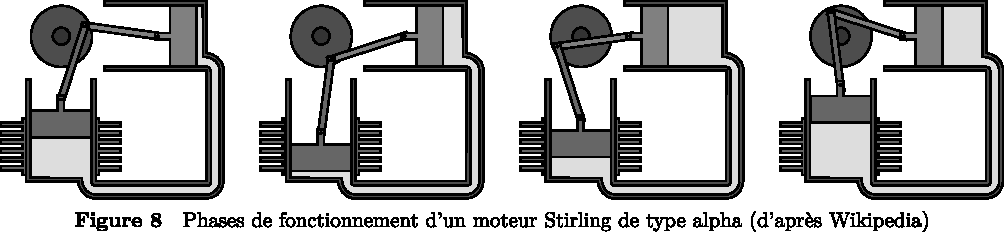
\includegraphics[width=17cm,height=\textheight]{images-DS9/pb-stirling-fig8.pdf}

\end{center}

Le mouvement du gaz peut être décrit par 4 phases plus ou moins
distinctes (figure 8) :

\begin{itemize}
\tightlist
\item
  une phase de compression, pendant laquelle le volume de la chambre
  chaude est minimal, le fluide, entièrement situé dans la zone froide,
  est comprimé par le piston de travail dans sa course vers le bas ;
\item
  une fois le piston de travail au point mort bas, le déplaceur est
  ramené à gauche, ce qui a pour effet de transvaser le fluide comprimé,
  qui passe de la zone froide vers la zone chaude et reçoit un transfert
  thermique de la source externe ;
\item
  une phase de détente, pendant laquelle le fluide se détend dans le
  volume d'expansion où il continue d'être chauffé. Cette détente a pour
  effet de repousser le déplaceur et le piston de travail ;
\item
  une fois que le piston de travail a atteint le point mort haut, le
  déplaceur est ramené à droite, ce qui a pour effet de transvaser le
  fluide de la zone chaude (volume d'expansion) vers la zone froide
  (volume de compression). Au cours de ce transfert, le fluide cède de
  la chaleur au refroidisseur.
\end{itemize}

Un cycle réel d'un moteur de Stirling est représenté dans le diagramme
\((p,V)\), \textbf{sur le document réponse à rendre avec la copie.}

\begin{enumerate}
\def\labelenumi{\arabic{enumi}.}
\tightlist
\item
  Justifier que ce cycle est celui d'un moteur. Estimer la valeur du
  travail fourni par le moteur pendant un cycle.
\end{enumerate}

\subsection*{Modélisation du cycle}\label{moduxe9lisation-du-cycle}
\addcontentsline{toc}{subsection}{Modélisation du cycle}

On étudie le cycle de Stirling idéal. Au cours de celui-ci, \(n\) moles
de gaz parfait de coefficient adiabatique \(\gamma\) subissent les
transformations suivantes :

\begin{itemize}
\tightlist
\item
  une compression \((1 \to 2)\) isotherme réversible à la température
  \(T_1\),
\item
  un échauffement \((2 \to 3)\) isochore jusqu'à l'état 3 de température
  \(T_3\),
\item
  une détente \((3 \to 4)\) isotherme réversible à la température
  \(T_3\),
\item
  un refroidissement \((4 \to 1)\) isochore jusqu'à l'état 1.
\end{itemize}

Il n'y a pas d'autre travail que celui des forces de pression.

\begin{enumerate}
\def\labelenumi{\arabic{enumi}.}
\setcounter{enumi}{1}
\tightlist
\item
  Représenter sur la figure du document réponse, à rendre avec la copie,
  l'allure du diagramme correspondant au cycle idéal.
\end{enumerate}

On note \(r = \frac{V_1}{V_2}\) le rapport de compression entre les
volumes fixés par construction. On rappelle que la capacité thermique à
volume constant d'un gaz de \(n\) moles de gaz parfait vaut
\(C_V=\frac{nR}{\gamma -1}\) où \(R\) est la constante des gaz parfaits.

\begin{enumerate}
\def\labelenumi{\arabic{enumi}.}
\setcounter{enumi}{2}
\item
  Exprimer \(W_{12}\) , le travail reçu par le fluide au cours de la
  compression, en fonction de \(n, R, T_1\) et \(r\). En déduire le
  transfert thermique \(Q_{12}\) reçu par le fluide au cours de cette
  compression en fonction de \(n, R, T_1\) et \(r\). Préciser les signes
  de \(W_{12}\) et de \(Q_{12}\) .
\item
  Exprimer \(Q_{23}\), le transfert thermique reçu par le fluide au
  cours de l'échauffement isochore, en fonction de \(n, R, T_1, T_3\) et
  \(\gamma\). Préciser son signe.
\item
  Exprimer \(W_{34}\) , le travail reçu par le fluide au cours de la
  détente, en fonction de \(n, R, T_3\) et \(r\). En déduire le
  transfert thermique \(Q_{34}\) reçu par le fluide au cours de cette
  détente en fonction de \(n, R, T_3\) et \(r\). Préciser les signes de
  \(W_{34}\) et \(Q_{34}\).
\item
  Exprimer le transfert thermique \(Q_{41}\) reçu par le fluide au cours
  du refroidissement en fonction de \(n, R, T_1 , T_3\) et \(\gamma\).
  Préciser son signe.
\end{enumerate}

\subsection*{Rendement du moteur}\label{rendement-du-moteur}
\addcontentsline{toc}{subsection}{Rendement du moteur}

\begin{enumerate}
\def\labelenumi{\arabic{enumi}.}
\setcounter{enumi}{6}
\item
  Définir puis exprimer le rendement idéal du moteur en fonction de
  \(T_1 , T_3 , r\) et \(\gamma\).
\item
  Définir et exprimer le rendement de Carnot en fonction de \(T_1\) et
  \(T_3\).
\end{enumerate}

Dans beaucoup de situations, le moteur de Stirling contient un
régénérateur. Dans ce cas, la chaleur perdue par le gaz lors du
refroidissement isochore \((4 \to 1)\) est récupérée par le gaz lors du
chauffage isochore \((2 \to 3)\). Si le régénérateur est idéal, cette
récupération est totale.

\begin{enumerate}
\def\labelenumi{\arabic{enumi}.}
\setcounter{enumi}{8}
\tightlist
\item
  Que devient le rendement du cycle idéal dans ce cas ?
\end{enumerate}

On considère 2 moteurs de Stirling combinés dont l'efficacité est
environ 50 \% de l'efficacité de Carnot, alimenté par une puissance
électrique d'environ 180 W.

\begin{enumerate}
\def\labelenumi{\arabic{enumi}.}
\setcounter{enumi}{9}
\tightlist
\item
  En prenant une température chaude de 640 °C et une température froide
  de 60 °C et en supposant la conversion du travail mécanique en travail
  électrique parfaite, estimer numériquement la puissance thermique
  fournie par la source chaude aux deux moteurs de Stirling combinés.
\end{enumerate}

\section*{Problème 2: Étude thermodynamique d'une chambre
froide}\label{probluxe8me-2-uxe9tude-thermodynamique-dune-chambre-froide}
\addcontentsline{toc}{section}{Problème 2: Étude thermodynamique d'une
chambre froide}

Le stockage des récoltes s'effectue dans une chambre froide. On se
propose dans cette partie d'étudier cette machine thermique. Le fluide
réfrigérant étudié est du R134a. Pour les futures constructions, le
fluide sera du R1234ze pour sa moindre contribution à l'effet de serre.

\subsection*{Généralités}\label{guxe9nuxe9ralituxe9s}
\addcontentsline{toc}{subsection}{Généralités}

Le fluide réfrigérant décrit le cycle thermodynamique présenté figure 8.
On modélise la machine frigorifique par une machine ditherme schématisée
en figure 9.

On utilise les notations suivantes :

\begin{itemize}
\tightlist
\item
  \(Q_c\) : transfert thermique algébriquement reçu par le fluide au
  cours d'un cycle de la part de la source chaude à la température
  \(T_c\);
\item
  \(Q_f\) : transfert thermique algébriquement reçu par le fluide au
  cours d'un cycle de la part de la source froide à la température
  \(T_f\);
\item
  \(W\) : travail algébriquement reçu par le fluide au cours d'un cycle
  de la part de l'extérieur.
\end{itemize}

\begin{center}

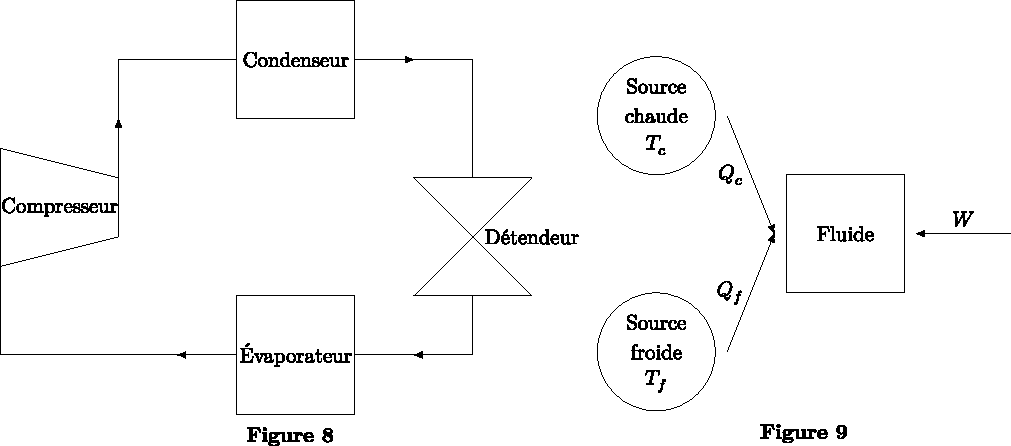
\includegraphics[width=17cm,height=\textheight]{images-DS9/pb-chambre-fig89.pdf}

\end{center}

\begin{enumerate}
\def\labelenumi{\arabic{enumi}.}
\item
  Au niveau de quel organe de la machine thermique se trouve la chambre
  froide ? Justifier votre réponse.
\item
  Préciser en justifiant les signes de \(Q_c,Q_f\) et \(W\).
\item
  Définir l'efficacité \(e\) (également appelé COefficient de
  Performance COP) de la machine frigorifique.
\item
  Établir l'expression de l'efficacité de Carnot \(e_c\), en fonction de
  \(T_c\) et \(T_f\). Que peut-on dire l'efficacité réelle \(e\) par
  rapport à l'efficacité de Carnot \(e_c\)?
\item
  Calculer numériquement \(e_c\) avec \(T_c = 45\ ^\circ\mathrm{C}\) et
  \(T_f = 3\ ^\circ\mathrm{C}\). Interpréter le résultat obtenu.
\end{enumerate}

\subsection*{Description du cycle}\label{description-du-cycle}
\addcontentsline{toc}{subsection}{Description du cycle}

Le cycle comprend les successions de transformations suivantes :

\begin{itemize}
\tightlist
\item
  \(1 \to 2\) : compression adiabatique réversible en phase gazeuse dans
  le compresseur ;
\item
  \(2 \to 3\) : refroidissement isobare de la vapeur ;
\item
  \(3 \to 4\) : compression totale et isobare ;
\item
  \(4 \to 5\) : sous-refroidissement isobare ;
\item
  \(5 \to 6\) : détente isenthalpique ;
\item
  \(6 \to 7\) : chauffage isobare ;
\item
  \(7 \to 1\) : surchauffe de la vapeur.
\end{itemize}

Le tableau 2 donne le relevé thermodynamique du fluide aux différents
points de ce cycle.

\begin{center}

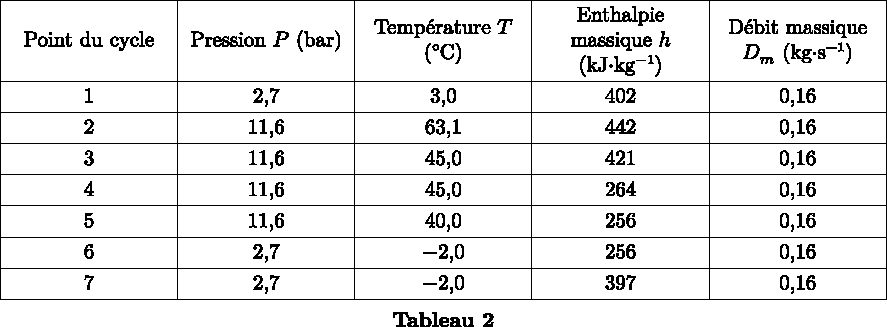
\includegraphics[width=15cm,height=\textheight]{images-DS9/pb-chambre-tab2.pdf}

\end{center}

\begin{enumerate}
\def\labelenumi{\arabic{enumi}.}
\setcounter{enumi}{5}
\item
  Représenter le cycle thermodynamique sur le diagramme des frigoristes
  \((p,h)\) du document réponse.
\item
  Qualifier l'état du fluide aux points 3 et 4.
\item
  Lire graphiquement le titre en vapeur \(x_v\) du point 6.
\item
  Rappeler l'expression du premier principe de la thermodynamique pour
  un fluide en écoulement stationnaire, dans lequel on néglige les
  variations d'énergie cinétique massique \(\Delta e_c\) et d'énergie
  potentielle de pesanteur massique \(\Delta e_p\) devant la variation
  d'enthalpie massique \(\Delta h\).
\item
  Exprimer puis calculer numériquement le transfert thermique massique
  \(q_f\) reçu par le fluide dans l'évaporateur.
\item
  Exprimer puis calculer numériquement le transfert thermique massique
  \(q_c\) reçu par le fluide dans le condenseur.
\item
  Exprimer puis calculer numériquement le travail indiqué \(w_i\) reçu
  par le fluide de la part du compresseur.
\item
  En déduire l'efficacité réelle \(e\) de la machine frigorifique.
\item
  Exprimer puis calculer numériquement la puissance thermique extraite
  de la chambre froide \(P_{th,f}\).
\end{enumerate}

\newpage

\section*{Problème 3: Étude de deux gaz parfaits dans un
cylindre}\label{probluxe8me-3-uxe9tude-de-deux-gaz-parfaits-dans-un-cylindre}
\addcontentsline{toc}{section}{Problème 3: Étude de deux gaz parfaits
dans un cylindre}

Deux gaz, supposés parfaits, sont enfermés dans deux compartiments (1)
et (2) séparés par un piston mobile athermane (on dit aussi calorifugé)
qui coulisse sans frottement. Le compartiment (1) est entièrement
calorifugé tandis que le compartiment (2) peut échanger de l'énergie par
chaleur (transfert thermique) avec le milieu extérieur, assimilé à un
thermostat de température \(T_0\) , à travers une paroi diathermane fixe
(non calorifugée).

Les deux compartiments contiennent chacun \(n\) moles de gaz et sont,
dans l'état initial, à la température \(T\) . Le volume total des deux
compartiments est \(V_t = 2V_0\) , où \(V_0\) désigne les volumes,
initialement égaux, de chacun des deux compartiments.

\begin{center}

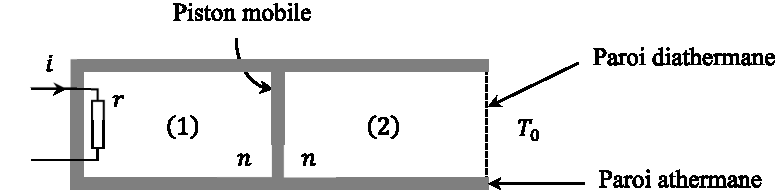
\includegraphics[width=12cm,height=\textheight]{images-DS9/pb-2gaz.pdf}

\end{center}

À un instant pris comme origine temporelle, le compartiment (1) reçoit
de la chaleur par l'intermédiaire d'un résistor (résistance \(r\))
alimentée pendant une durée \(\tau\), par un générateur qui délivre un
courant d'intensité \(i\) constante.

L'état final est l'état d'équilibre thermodynamique du système qui
succède à ce chauffage. On le caractérise par les variables d'état
\(P_k , V_k\) et \(T_k\) qui représentent les pressions, volumes et
températures des compartiments \((k)\) où \(k = 1\) ou \(2\).

On note \(R\) la constante des gaz parfaits et
\(\gamma = \frac{C_{pm}}{C_{vm}}\) le rapport de la capacité thermique
molaire à pression constante sur la capacité thermique molaire à volume
constant, identique pour les gaz des deux compartiments.

\begin{center}

\textbf{Indiquer la (ou les) bonne(s) réponse(s) en justifiant tout
votre raisonnement.}

\end{center}

\begin{enumerate}
\def\labelenumi{\arabic{enumi}.}
\item
  Exprimer \(V_1\) et \(V_2\)
  \[ A) \ V_1 = \frac{T_1}{T_0 + T_1}V_0 \qquad\qquad B) \ V_1 = \frac{T_1}{T_0 + T_1}V_t \ \qquad\qquad C) \ V_2 = \frac{T_0}{T_0 + T_1}V_0 \qquad\qquad D) \ V_2 = \frac{T_0}{T_0 + T_1}V_t\]
\item
  Que peut-on affirmer ?
  \[ A) \ P_1 = P_2 \qquad\qquad B) \ P_1 = \frac{nR(T_0 + T_1)}{V_t} \ \qquad\qquad C) \ P_1 = \frac{nR(T_0 + T_1)}{V_0} \qquad\qquad D) \ P_1 \neq P_2\]
\item
  Déterminer la variation d'énergie interne \(\Delta U\) entre l'état
  initial et l'état final du système constitué par les deux gaz (on
  indique que \(\Delta U\) est la somme des variations des énergies
  internes des deux gaz, entre l'état initial et final) :
  \[ A) \ \Delta U = 0 \qquad\qquad B) \ \Delta U = \frac{nR}{\gamma -1}(T_1 - T_0) \ \qquad\qquad C) \ \Delta U = \frac{nR\gamma}{\gamma -1}(T_1 - T_0) \qquad\qquad D) \ \Delta U = nR(T_1 - T_0)\]
\end{enumerate}

\emph{On supposera dans toute la suite que la transformation du
compartiment (2) est réversible.}

\begin{enumerate}
\def\labelenumi{\arabic{enumi}.}
\setcounter{enumi}{3}
\item
  On note \(W\) et \(Q\) le travail et la chaleur (transfert thermique)
  algébriquement reçus par le gaz du compartiment (2) entre l'état
  initial et l'état final. Que peut-on affirmer ?
  \[ A) \ W_2 = nRT_0\ln\left(\frac{T_0 + T_1}{2T_0}\right) \qquad\qquad B) \ W_2 = 0 \ \qquad\qquad C) \ Q_2 = 0 \qquad\qquad D) \ Q_2 = -W_2\]
\item
  On note \(Q\) la chaleur (transfert thermique) algébriquement reçu par
  le gaz du compartiment (1) entre l'état initial et l'état final. Que
  peut-on affirmer ?
  \[ A) \ Q_1 = \Delta U \qquad\qquad B) \ Q_1 = \Delta U + W_1 \ \qquad\qquad C) \ Q_1 = W_2 \qquad\qquad D) \ Q_1 = ri^2\tau\]
\end{enumerate}

On note \(S_2^{(r)}\) l'entropie algébriquement reçue et \(S_2^{(c)}\)
l'entropie algébriquement créée, entre l'état initial et l'état final,
pour le gaz situé dans le compartiment (2). On indique que sa variation
d'entropie \(\Delta S_2\) entre l'état initial et l'état final s'écrit
\(\Delta S_2 = nR \ln\left(\frac{V_2}{V_0}\right)\).

\begin{enumerate}
\def\labelenumi{\arabic{enumi}.}
\setcounter{enumi}{5}
\tightlist
\item
  Exprimer \(S_2^{(r)}\) et \(S_2^{(c)}\)
  \[ A) \ S_2^{(r)} = nR\ln\left(\frac{2T_0}{T_0 + T_1}\right) \qquad\qquad B) \ S_2^{(r)} = 0 \ \qquad\qquad C) \ S_2^{(c)} = nR\ln\left(\frac{2T_0}{T_0 + T_1}\right) \qquad\qquad D) \ S_2^{(c)} = 0\]
\end{enumerate}

\section*{Problème 4: Cycle de
Carnot}\label{probluxe8me-4-cycle-de-carnot}
\addcontentsline{toc}{section}{Problème 4: Cycle de Carnot}

\subsection*{Chaleur perdue et machine
thermique}\label{chaleur-perdue-et-machine-thermique}
\addcontentsline{toc}{subsection}{Chaleur perdue et machine thermique}

Les enjeux de la transition énergétique amènent des réflexions sur
l'efficacité des systèmes de production et de conversion de l'énergie,
ainsi que sur la récupération d'énergie. Optimiser les systèmes de
production d'énergie et récupérer le plus d'énergie possible lors d'une
conversion d'énergie deviennent des sujets majeurs dans le cadre d'une
politique d'économie d'énergie.

Lors du fonctionnement d'un procédé industriel, l'énergie thermique
produite grâce à l'énergie apportée n'est pas utilisée en totalité. Une
partie de la chaleur est inévitablement rejetée et non récupérée. En
raison de ce caractère inéluctable, on parle de \emph{chaleur fatale}.
Cette quantité d'énergie perdue constitue un gisement potentiel à
récupérer.

Cependant, cette appellation est en partie erronée car la chaleur fatale
peut être en partie récupérée. L'ADEME (Agence De l'Environnement et de
la Maı̂trise de l'Energie) classe le gisement de chaleur fatale
disponible par écart de température par rapport à la température
ambiante (source froide).

Le tableau ci-dessous donne les gisements de chaleur fatale (Énergie
thermique) disponible par an et classés par écart de température avec la
température ambiante, ici prise à 27°C.

\begin{longtable}[]{@{}cc@{}}
\toprule\noalign{}
Écart de température & Gisement \\
\midrule\noalign{}
\endhead
\bottomrule\noalign{}
\endlastfoot
\(30\ ^\circ\mathrm{C}\) & \(20\ \mathrm{TWh}\) \\
\(75\ ^\circ\mathrm{C}\) & \(20\ \mathrm{TWh}\) \\
\end{longtable}

\begin{enumerate}
\def\labelenumi{\arabic{enumi}.}
\tightlist
\item
  Rappeler l'expression du premier principe et du deuxième principe de
  la thermodynamique. Que deviennent ces expressions sur un cycle
  thermodynamique ?
\end{enumerate}

On considère un système thermodynamique quelconque, noté
\(\mathcal{S}\), en contact avec deux thermostats aux températures
\(T_\mathrm{ch}\) et \(T_\mathrm{fr}\) avec
\(T_\mathrm{ch} > T_\mathrm{fr}\). On note \(Q_C\) la chaleur échangée
entre le système \(\mathcal{S}\) et la source \(T_\mathrm{ch}\) , et
\(Q_F\) la chaleur échangée entre le système \(\mathcal{S}\) et la
source \(T_\mathrm{fr}\).

\begin{enumerate}
\def\labelenumi{\arabic{enumi}.}
\setcounter{enumi}{1}
\item
  Rappeler le nom et la définition des transformations associées à un
  cycle de Carnot subi par le système \(\mathcal{S}\), en contact avec
  les deux thermostats précédents. On représentera les étapes du cycle
  dans le plan \((T,S)\) en faisant apparaitre clairement les
  températures des thermostats.
\item
  Dans le cas d'un système subissant un cycle de Carnot, réaliser un
  bilan d'énergie et un bilan d'entropie, et en déduire l'expression du
  rendement \(\eta\) en fonctionnement moteur en fonction de
  \(T_\mathrm{ch}\) et \(T_\mathrm{fr}\).
\item
  À partir des données du tableau précèdent, justifier pourquoi l'ADEME
  classe les gisements par écart de température par rapport à la
  température de la source froide et en déduire en Wh l'énergie que l'on
  pourrait récupérer par an et par gisement.
\end{enumerate}

\subsection*{Machine de Carnot opérée avec un gaz
parfait}\label{machine-de-carnot-opuxe9ruxe9e-avec-un-gaz-parfait}
\addcontentsline{toc}{subsection}{Machine de Carnot opérée avec un gaz
parfait}

Considérons le système \(\mathcal{S}\) précédent comme étant un gaz
parfait et subissant un cycle de Carnot entre \(T_\mathrm{ch}\) et
\(T_\mathrm{fr}\) , respectivement à 57°C et 27°C. À chaque état du
cycle, le volume, la pression et la température du système
\(\mathcal{S}\) sont indicés successivement par 1, 2, 3 et 4.

L'état 1 du cycle correspond au moment juste avant la phase de
compression adiabatique. Dans cet état, le système est dans un volume de
1 cm × 1cm × 1mm (noté \(V_1\)), la pression est de 1 bar (notée
\(P_1\)) et sa température est \(T_1 = T_\mathrm{fr}\) . On notera que
sur la phase d'échange de chaleur avec la source chaude, la variation de
pression est de 0,4 bar.

On note \(c_p\) et \(c_v\) les capacités thermiques massiques du système
à pression constante et à volume constant, respectivement, en
\(\mathrm{J.K^{-1}.kg^{-1}}\). On rappelle que ces capacités thermiques
obéissent à la relation de Mayer : \(c_p - c_v = \frac{R}{M}\), où \(R\)
est la constante universelle des gaz parfaits, et \(M\) la masse
molaire. On considère dans la suite que le système \(\mathcal{S}\) est
constitué d'air, assimilé à un gaz parfait diatomique, tel que l'indice
adiabatique \(\gamma = \frac{c_p}{c_v}\) vaut 7/5.

\begin{enumerate}
\def\labelenumi{\arabic{enumi}.}
\setcounter{enumi}{4}
\item
  Caractériser qualitativement la variation de pression du système
  \(\mathcal{S}\) le long du cycle, en détaillant les transformations
  entre chaque état thermodynamique: \(1 \to 2, 2 \to 3, 3 \to 4\) et
  \(4 \to 1\).
\item
  Donner l'expression de la dérivée \(\derive{P}{V}\) pour chaque
  transformation en fonction de \(\gamma, P\) et \(V\) et représenter
  les étapes du cycle dans le plan \((P,V)\).
\end{enumerate}

Pour un gaz parfait, la variation infinitésimale d'entropie
\(\mathrm{d} S\) s'exprime en fonctions des variations infinitésimales
de température \(\mathrm{d} T\) et de pression \(\mathrm{d} P\):
\[\mathrm{d}S = \frac{m c_p}{T} \mathrm{d}T - \frac{nR}{P}\mathrm{d}P \]
avec \(n\) la quantité de matière et \(m\) la masse du gaz.

\begin{enumerate}
\def\labelenumi{\arabic{enumi}.}
\setcounter{enumi}{6}
\item
  Exprimer \(\mathrm{d}S\) en fonction en fonction de
  \(P_1 , V_1, T_1\), et des capacités thermiques massiques. On ne fera
  pas intervenir dans le résultat \(n\) et \(m\).
\item
  Calculer les valeurs numériques des pressions \(P_1,P_2,P_3\) et
  \(P_4\).
\item
  Exprimer les chaleurs échangées \(Q_\mathrm{ch}\) en fonction de
  \(P_1 , V_1, T_1, T_\mathrm{ch}, P_2/P_3\) et \(Q_\mathrm{fr}\) en
  fonction de \(P_1 , V_1 , T_1, T_\mathrm{fr} , P_4/P_1\). Évaluer
  numériquement \(Q_\mathrm{ch}\) et \(Q_\mathrm{fr}\).
\item
  En déduire l'expression et la valeur numérique du travail mécanique
  récupéré pour un cycle moteur. Le résultat paraît-il cohérent avec la
  valeur obtenue si on utilise l'expression du rendement de Carnot ?
\item
  Les machines thermiques de récupération de chaleur fatale fonctionnent
  en réalité avec deux transformations isobares pour des raisons
  techniques. Expliquer pourquoi un fluide subissant une transition de
  phase (un changement d'état ici) permet d'améliorer l'efficacité de la
  machine thermique.
\end{enumerate}

%% Document réponse à rendre (doit être en page impaire!)
\newpage

\begin{tcolorbox}
\centering\huge{\textbf{Document réponse \\\emph{A rendre avec la copie}}}
\end{tcolorbox}

\textbf{Nom: \hspace{7cm} Prénom:}\\

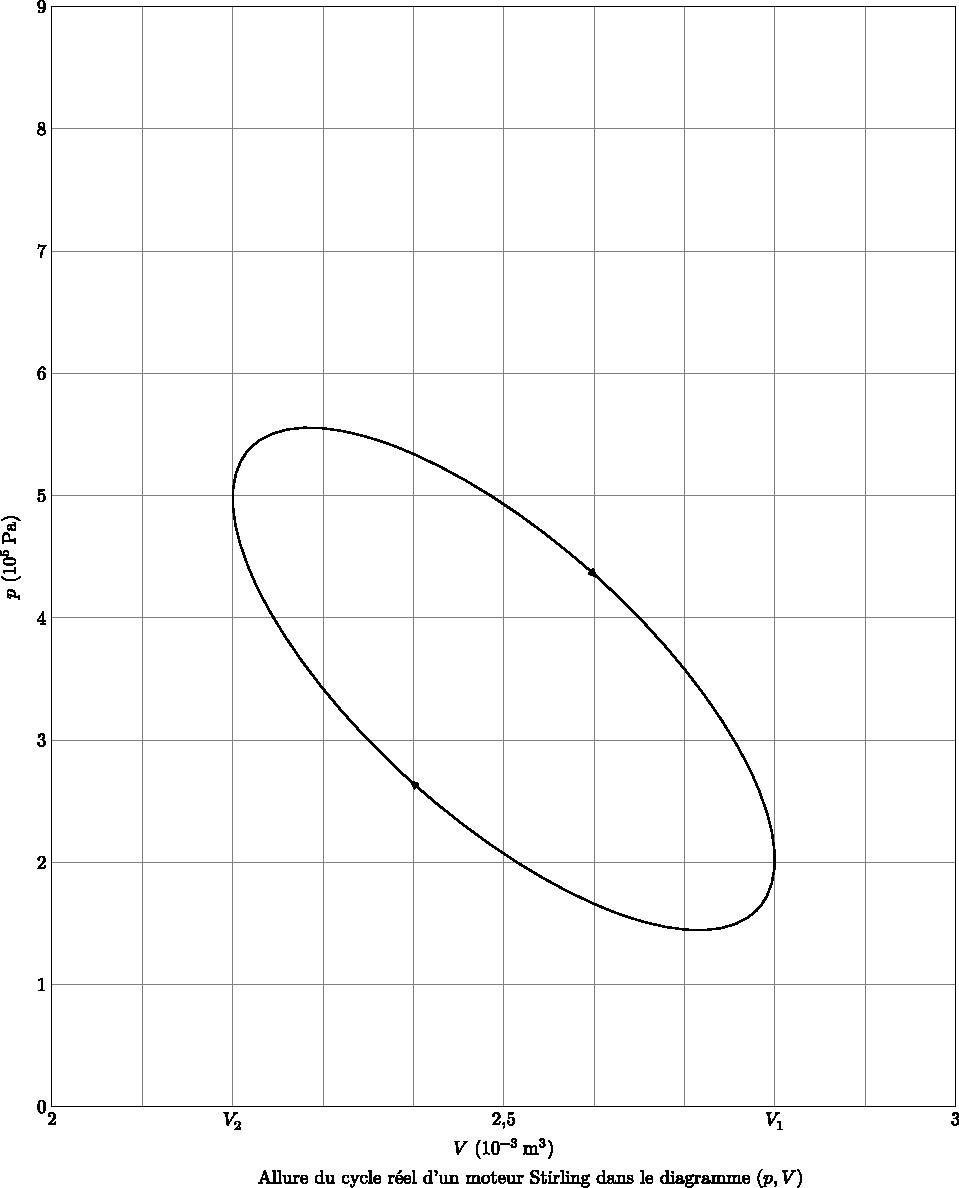
\includegraphics[width=17cm,height=\textheight]{images-DS9/pb-stirling-cycle.pdf}

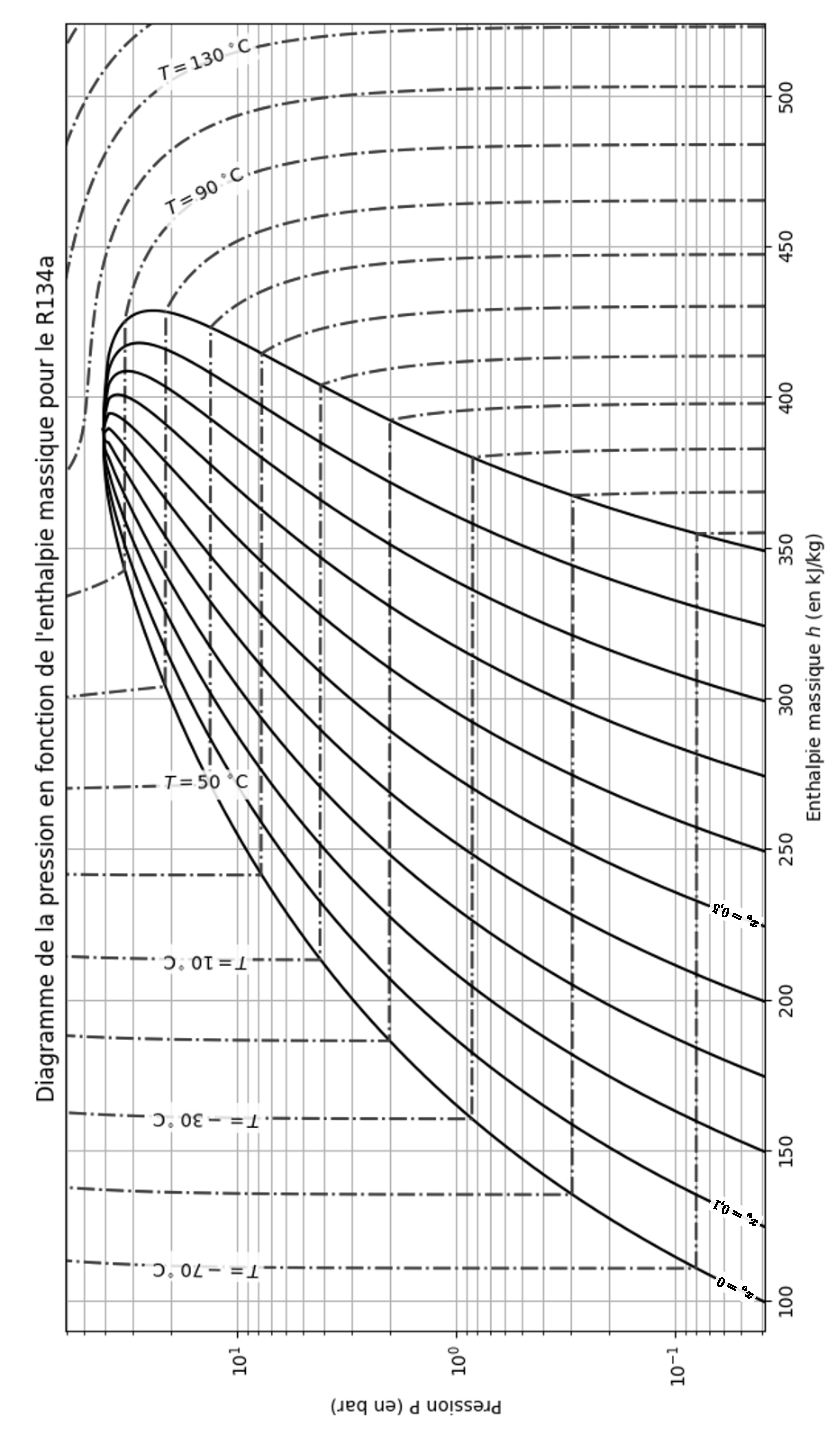
\includegraphics[width=16.5cm,height=\textheight]{images-DS9/pb-chambre-ph.pdf}


\end{document}
